\documentclass[11pt]{article}
\usepackage{graphicx}
\usepackage{float}
\title{\textbf{CS427/527\\
               An Introduction to Artifical Intelligence\\
               Homework 3 (Chapter 4)}}
\author{Jacob Hurst}
\date{\today}

\begin{document}

\maketitle

\section{The sliding-tile puzzle consists of three black tiles, three white tiles, and an empty space in the given configuration.
\\\\The puzzle has two legal moves with associated costs:
\\1. A tile may move into an adjacent empty location. This has a cost of 1.
\\2. A tile can hop over one or two other tiles into the empty position. This has a cost equal to the number of tiles jumped over.
\\\\The goal is to have all the white tiles to the left of all the black tiles. The position of the blank is not important.
\\1. Analyze the state space with respect to complexity and looping.
\\2. Propose a heuristic for solving this problem and analyze it with respect to admissibility, monotonicity, and informedness.}

\begin{enumerate}
	\item The number of branches from each state is dependent on the location of the empty space. 
	\\If the empty space is in the middle of the configuration, then we can branch out to 6 different states (enumerating BBB-WWW, we have, BB-BWWW, B-BBWWW, -BBBWWW, BBBW-WW, BBBWW-W, and BBBWWW-). 
	\\If the empty space is off by one from the center, then we can branch out to 5 different states (enumerating BB-BWWW since BBBW-WW is similar; we have, BBB-WWW, B-BBWWW, -BBBWWW, BBWB-WW, and BBWBW-W). 
	\\If the empty space is off by two from the center, then we can branch out to 4 different states (enumerating B-BBWWW since BBBWW-W is similar; we have, -BBBWWW, BB-BWWW, BBB-WWW, and BWBB-WW). 
	\\If the empty space is off by three from the center, then we can branch out to 3 different states (enumerating -BBBWWW since BBBWWW- is similar; we have, B-BBWWW, BB-BWWW, and BBB-WWW). 
	\\The minimum branching factor for a state is 3. The maximum branching factor for a state is 6. 
	\\Any child state can loop back to it's parent state (and possibly to it's grandparent state), we can maintain a closed list of visited states to avoid looping. 
	\\The complexity of the state space is $6!$ as we have $6*4*3$ possible states for one side of the state space and  $6*4*3*2$ for both sides of the state space.
	\item One possible heuristic is to count the number of tiles out of place from the goal position(s). This can be achieved by counting the W tiles to the right of each B tile. Analyzing this heuristic.
	\\Admissibility: This heuristic is admissible as, at each step, it will first explore the path that minimizes the count of W tiles to the right of each B tile. This will lead to a minimal path to a solution as the solutions that involve higher counts of W tiles to the right of each B tile will be set aside.
	\\Monotonicity: This heuristic has the property that $h($goal$) = 0$, but $h(n_i) - h(n_j) \leq cost(n_i, n_j)$ is not necessarily true. Due to looping in the state space, it is possible for the $n_j$ state to be 'worse off' or farther from the goal than the $n_i$ state. If we maintain a list of closed states, we can improve on this but the heuristic itself does not guard against this. 
	\\Informedness: This heuristic may not be the most informed heuristic but it is more informed than performing a simple breadth-first search as the rule of this heuristic will explore the seemingly more promising states before the seemingly less promising states.
\end{enumerate}
 
\section{Perform minimax, left-to-right alpha-beta pruning, and right-to-left alpha-beta pruning on the tree below.}

\begin{figure}[H]
\centering
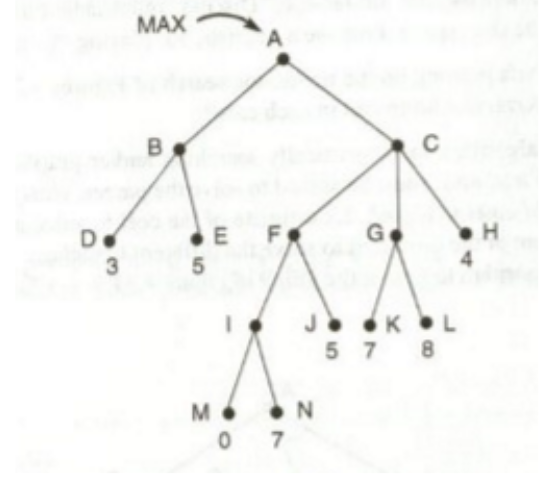
\includegraphics[scale=.5]{btree.png}
\caption{The tree in question}
\end{figure}

\subsection{Minimax}

\begin{figure}[H]
\centering
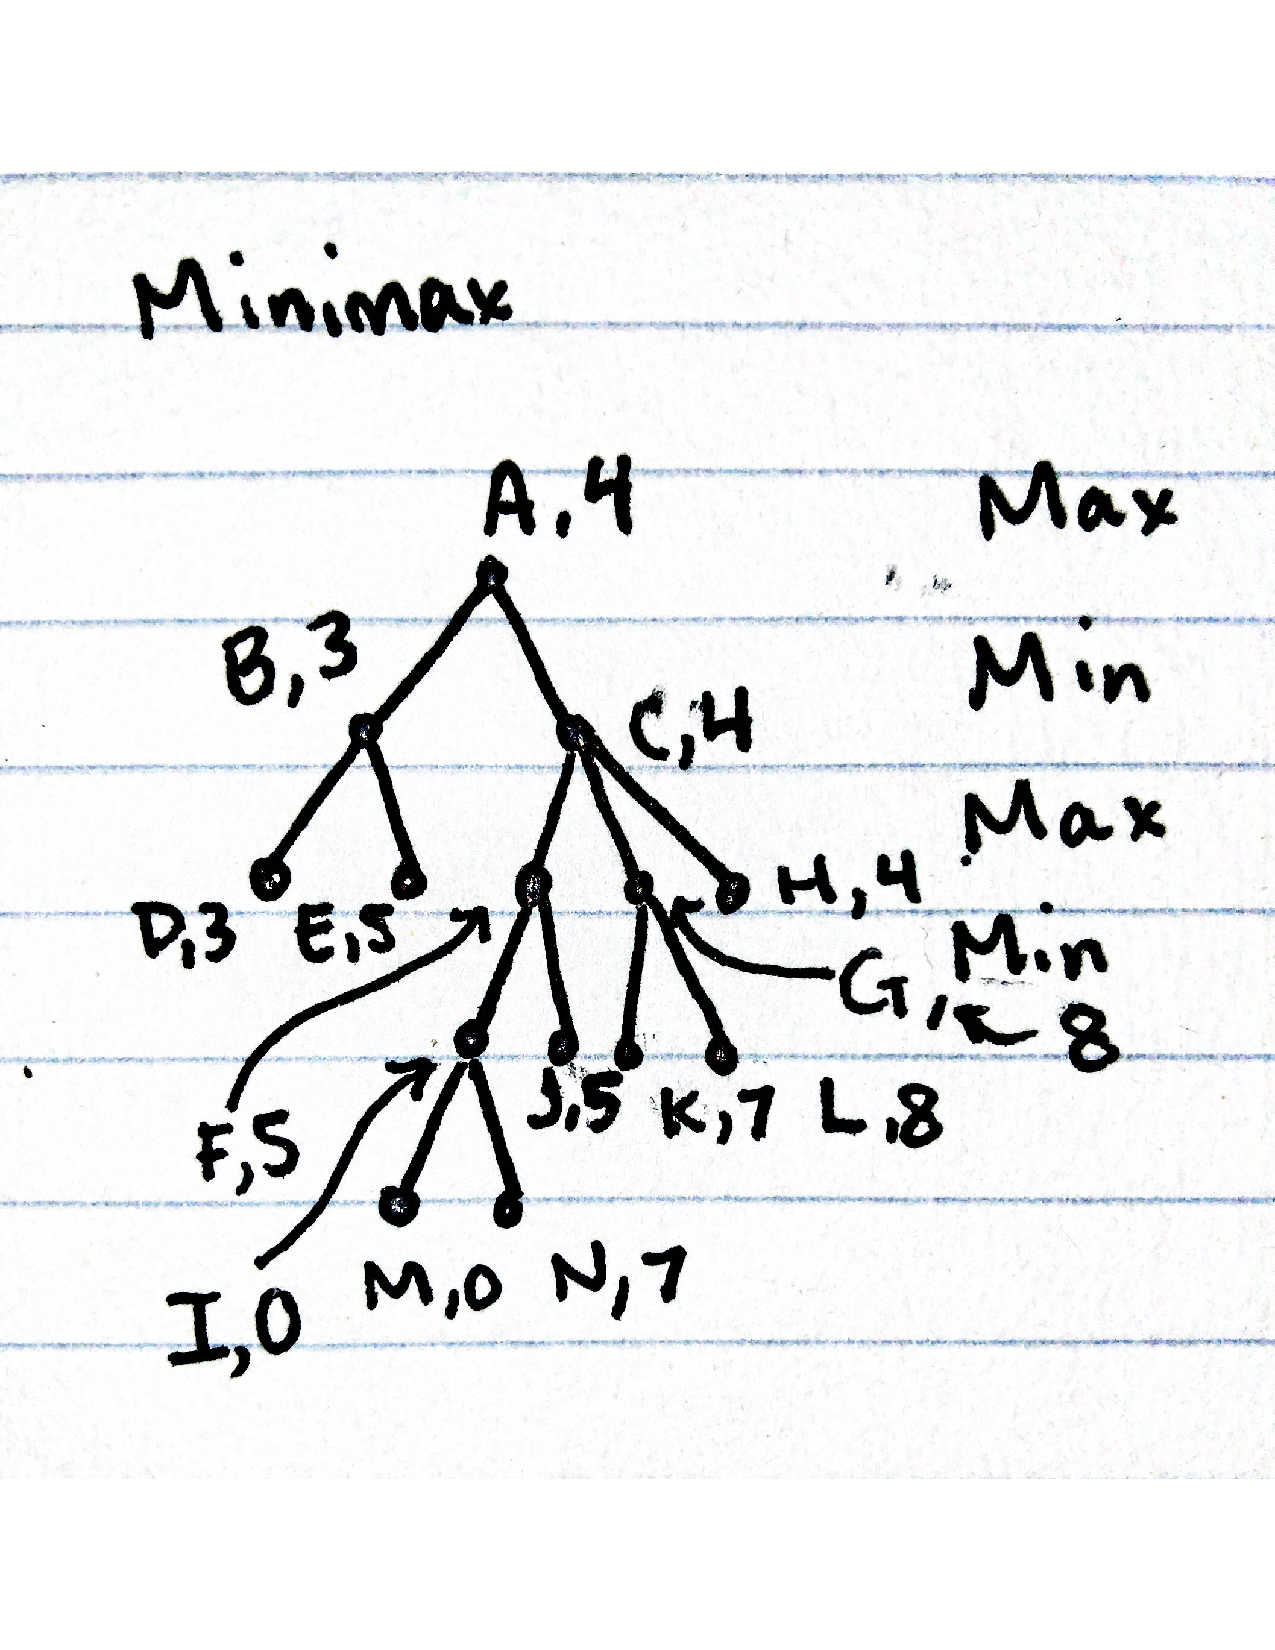
\includegraphics[scale=.5]{minimax.pdf}
\end{figure}

\subsection{Left-to-right $\alpha-\beta$ pruning}

\begin{figure}[H]
\centering
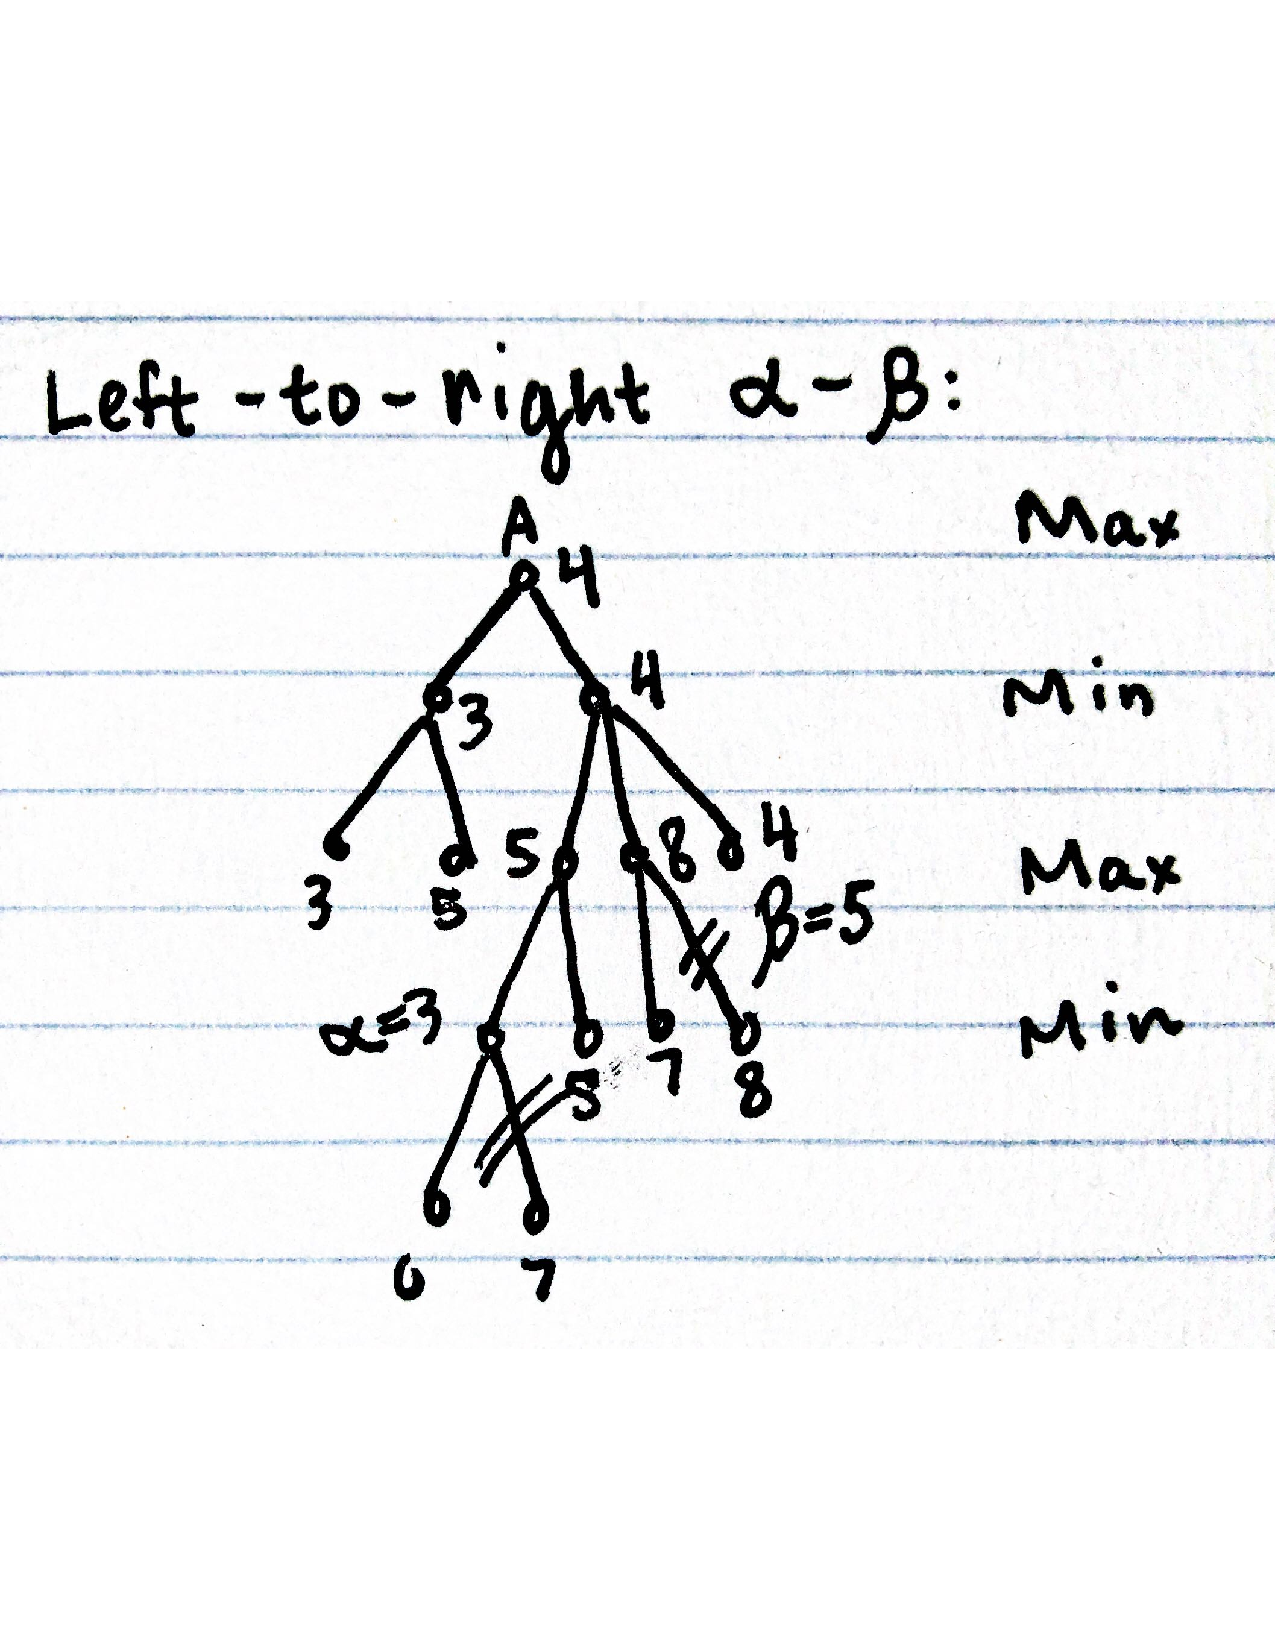
\includegraphics[scale=.5]{ltor.pdf}
\end{figure}

\subsection{Right-to-left $\alpha-\beta$ pruning}

\begin{figure}[H]
\centering
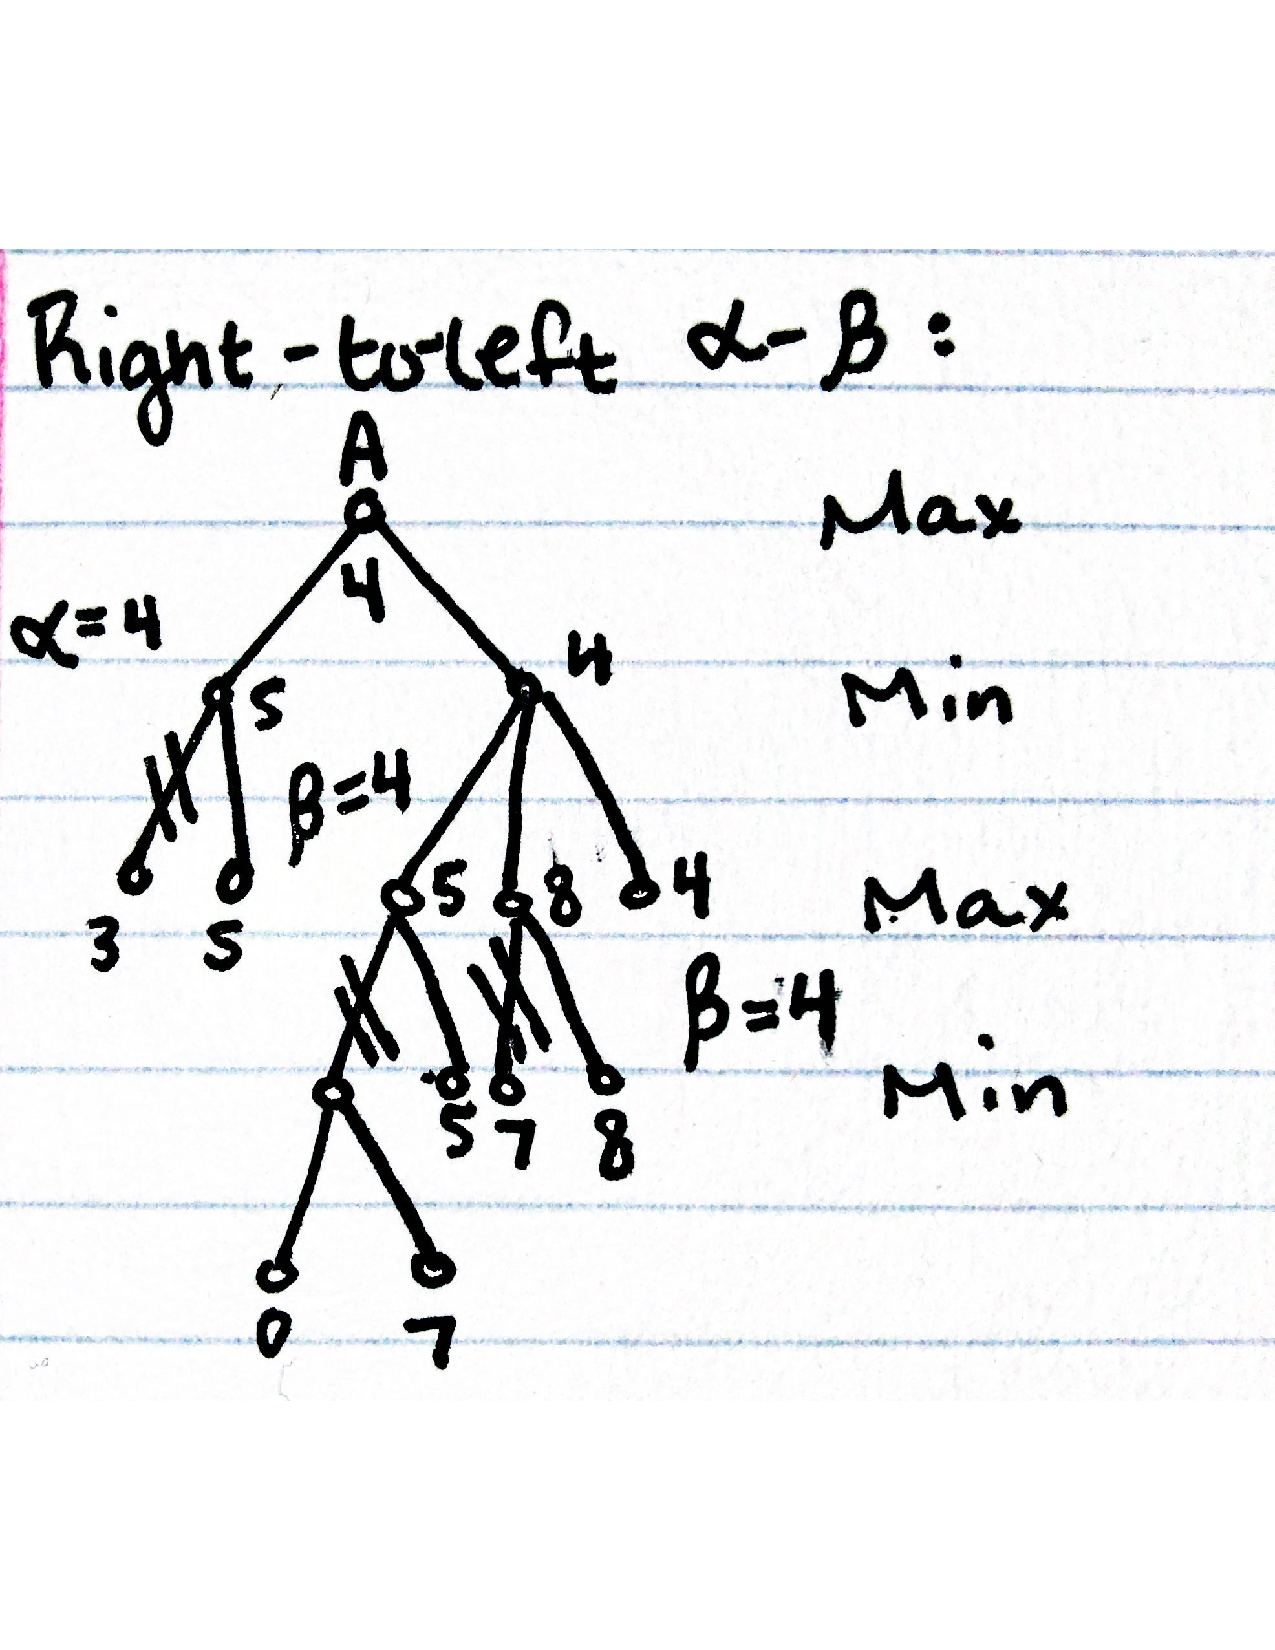
\includegraphics[scale=.5]{rtol.pdf}
\end{figure} 

\subsection{Discussion on pruning differences}

The differences in left-to-right versus right-to-left occur because of the differences in what has been seen and stored for alpha-beta values so far while traversing the tree. The ordering in which nodes are visited matter, if we visit the more promising nodes first (like we did in the right-to-left traversal) we might prune more often.

\end{document}